\documentclass{standalone}
\usepackage{tikz}
\usetikzlibrary{patterns,decorations.pathmorphing}
\begin{document}
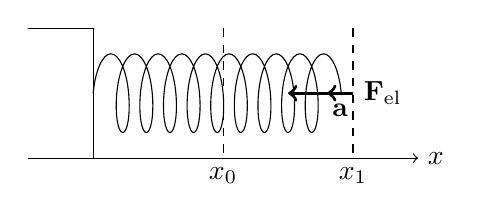
\begin{tikzpicture}[scale=1.65]
    \draw[->](-0.5,0)--(2.5,0)node[right]{$x$};
    \draw[-](0,0)--(0,1);
    \draw[-](0,1)--(-0.5,1);
    
    \draw[dashed](1,1)--(1,0)node[below]{$x_0$};
    \draw[dashed](2,1)--(2,0)node[below]{$x_1$};

    \draw[decoration={aspect=0.3, segment length=3mm, amplitude=5mm,coil},decorate] (0,0.5) -- (2,0.5); 
    \draw[->,very thick](2,0.5)node[right]{$\mathbf{F}_{\mathrm{el}}$}--(1.5,0.5);
    \draw[->,very thick](2,0.5)--(1.8,0.5)node[midway, below]{$\mathbf{a}$};
\end{tikzpicture}
\end{document}